\chapter{アプリケーションを作成する}

第6章コンポーネントの作成では、コンポーネントを作成し、APIを定義し、core.asyncチャンネルで接続する方法を学びました。今度は、これらのコンポーネントを実際のアプリケーションに組み入れる方法について見ていきましょう。

まず、ある問題を取り上げ、それをコンポーネントサイズの断片に分割する方法について考えます。次に、各コンポーネントの状態とAPIを定義し、最後にそれらを組み合わせてアプリケーションにします。

各コンポーネントは独自の設定データを持っています。開発時と様々なデプロイメント環境の両方で役立つように、1つ以上の外部ソースから設定をロードするための戦略を定義する必要があります。ここでは、設定を支援する2つのライブラリについて検討します。

まず、問題をどのようにコンポーネントに分割するかを決定することから始めましょう。

\section{モノを分解する}

最初の仕事は、問題からその問題を解決するための大まかなアーキテクチャに至るまで、どのようにすればよいかを考えることです。第6章「コンポーネントの作成」で説明したように、問題を分析し、個別のコンポーネントを特定します。アプリケーション内 (あるいは複数のアプリケーションにまたがる) で汎用的なコンポーネントを再利用したり、チーム内で開発を分担したり、あるいは一度に問題の一部だけを考えることができるような構造にしたりするためです。

コンポーネントを分離する方法にルールはありませんが、いくつかの一般的なガイドラインに従うことは可能です。コードをグループ化する理由としては、関数が同じ種類のデータで動作する、データの範囲や寿命が共通である、外部要件による変更の可能性が似ている、必要なリソースが似ている、などがあります。もし、あるコードのセットが、複数のコンテキストで異なる設定をしたときに再利用可能であれば、それは間違いなく有用なコンポーネントである。

この議論を具体化するために、次のような問題を考えてみよう。私たちの会社は、ソーシャルメディア上の製品に関する言及を監視し、それに対応できるシステムを必要としています。その応答は、タイムリーで、有用で、適切であることが重要である。この役割を果たす人はいますが、当社の製品は非常に人気があるため、注意が必要なメッセージを見つけ、回答候補を作成し、その回答を送信するというプロセスを自動化するための支援が必要です。

この問題を考えているうちに、アプリケーションにいくつかの境界線が見えてきました。ソーシャルメディアフィードの監視を自動化する場合、各サードパーティシステムとのやり取りをカプセル化するコンポーネントが必要です。これらのフィードは、個々のシステムとのやり取りは別々であっても、それ自体は多くの類似した実装ニーズを共有することができます。フィードは、外部リソースを使用し、そのライフサイクルをフィードに結合しているため、別個のコンポーネントとなります。

同様に、メッセージにどのように応答するかというルールの知識ベースをカプセル化するコンポーネントが必要になります。これは自己完結型でも、外部システムを使ってルールを呼び出すことも可能です。

最後に、元のメッセージと応答候補を受け取り、それらをソーシャルメディアの専門家に提示して、メッセージを承認するか修正するかを決定するコンポーネントが必要になると思われます。このコンポーネントは、ある人物へのアクセスを処理する役割を担っています。

アーキテクチャとそのハイレベルなコンポーネントがどのようなものかは、スケッチでご覧いただけます。 

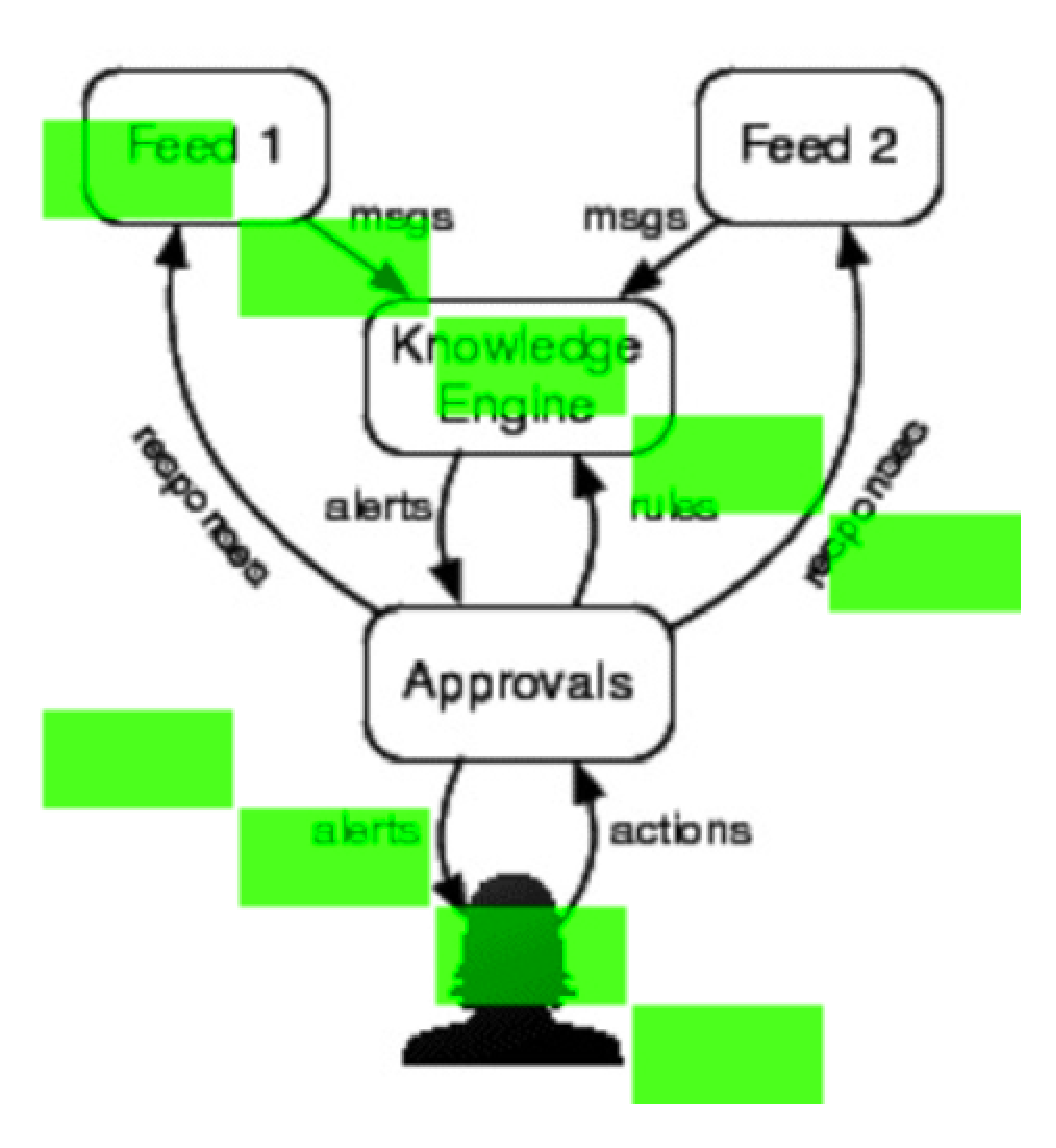
\includegraphics[width=8cm]{fig_07_001.eps}

次に、必要となるコンポーネントを定義し、それらをどのように接続するかを考えてみましょう。システムを組み立てていく上で、アプリケーションやコンポーネントのライフサイクルを考慮する必要がある。Clojureでこのような問題に最適なライブラリはComponentです\[20\]。コンポーネントを定義しながら、Componentを介してライフサイクルの開始と停止の機能を設定します。









 % Taking Things Apart
\section{Componentを用いた実装}

各コンポーネントについて、必要な構成、実行時の状態、他のコンポーネントとの接続を考慮する必要があります。コンポーネントとそのライフサイクルメソッドを定義したら、コンポーネントをどのように組み立てて実行システムにするかを見ていきましょう。

まず、ソーシャルメディアのフィードから始めましょう。各フィードには、そのフィードに接続するための認証設定が必要です。システムによっては、ユーザー名やパスワード、その他のアクセスキーが必要になります。また、フィードをアクティブにするか一時停止するかという実行時の状態も維持することになります。最後に、新しいメッセージを core.async チャネルでプッシュし、送信メッセージを別のチャネルで受信することを想定しています。このような情報を持つレコードとして、コンポーネントを定義します。


\begin{lstlisting}[numbers=none]
(defrecord Feed [auth status msg-chan response-chan])

(defn new-feed [auth msg-chan response-chan]
  (->Feed auth (atom :init) msg-chan response-chan))
\end{lstlisting}

最初の\texttt{auth}フィールドは、フィードタイプに指定された認証情報のマップを含む。\texttt{status}は、変化する実行時の状態です(アトムに保持されます)。最後の2つのフィールドは、メッセージの送信と受信に使用する実行時チャネルです。これらは起動時に接続され、その後変更されることはありません。

次に、\texttt{component/Lifecycle} プロトコルを実装してフィードの定義を拡張する必要があります。まず、Component をプロジェクトに追加し、以下の依存関係を設定します。

\begin{lstlisting}[numbers=none]
[com.stuartsierra/component "0.2.3"]
\end{lstlisting}

次に、名前空間に以下のrequireを追加します。

\begin{lstlisting}[numbers=none]
[com.stuartsierra.component :as component]
\end{lstlisting}

そして、コンポーネントの開始と停止のための2つのメソッドだけを持つ、\texttt{component/Lifecycle}プロトコルを拡張することができるようになりました。

\begin{lstlisting}[numbers=none]
(defrecord Feed [auth status msg-chan response-chan]
  component/Lifecycle
  (start [component]
    (reset! (:status component) :running)
    (process-messages status msg-chan)
    (handle-responses status response-chan)
    component)
  (stop [component]
    (reset! (:status component) :stopped)
    component))
\end{lstlisting}

\texttt{start}関数は、コンポーネントの状態を\texttt{:running}に設定し、受信メッセージを\texttt{msg-chan}に流す処理を開始し、応答を\texttt{response-chan}のフィードに戻す処理を開始します。サブプロセスはいずれもステータスを受け取り、ステータスが\texttt{:running}から変化したときに自分自身を停止させることができます。最後に、この関数は残りの起動のために同じコンポーネントのインスタンスを返します。

\texttt{stop}関数はステータスを\texttt{:stopped}に設定するだけです。残りの部分はサブプロセスが処理します。

次に、ナレッジエンジンコンポーネントを考えてみましょう。知識エンジンは、ルールの外部データベースに対する認証情報と、使用するルールセットで構成されます。実行時の状態は、外部のルール・データベースへの接続で構成されます。また、このコンポーネントにはフィードコンポーネントからの受信チャンネルと、承認コンポーネントへの送信フィードが必要です。

\begin{lstlisting}[numbers=none]
(defrecord KnowledgeEngine
  [ke-config feed-chan alert-chan rules]
  component/Lifecycle
  (start [component]
    (watch-feeds feed-chan alert-chan)
    component)
  (stop [component]
    component))

(defn new-knowledge-engine
  "初期ルールのない新しい知識エンジンを作成する"
  [ke-config feed-chan alert-chan]
  (->KnowledgeEngine ke-config feed-chan alert-chan
                     (atom (:rule-set ke-config))))
\end{lstlisting}

\texttt{KnowledgeEngine} コンポーネントは、コンポーネント構成データ、受信 \texttt{feed-chan} 、送信 \texttt{alert-chan} を保持するための \texttt{ke-config} を持ちます。さらに、この実装では、内部 \texttt{rules} を持ちます。これは、コンストラクタで公開されない実装の詳細です。他の実装では、外部のデータベースやルールシステムでルールを管理することができます。

知識エンジンの \texttt{start} 関数は、送られてくるフィードを監視し、ルールを処理し、必要と判断されればアラートチャンネルでアラートメッセージを発するプロセスをセットアップします。\texttt{stop} 関数は特別なことをする必要はありませんが、サブプロセスを停止させることは可能です。

知識エンジンは、ルールセットを管理するために、承認コンポーネントから直接呼び出すことができるAPIを持っています。回答を承認する人は、ナレッジエンジンから出力される内容に基づいてルールを追加、修正、削除することもでき、最終的にシステム全体を向上させることができます。ルールを追加するためのAPI関数の例は次のとおりです。

\begin{lstlisting}[numbers=none]
(defn add-rule
  "セットへのルール追加"
  [ke rule]
  (swap! (:rules ke) conj rule))
\end{lstlisting}

\texttt{add-rule}のようなコンポーネント関数は、通常、第一引数としてコンポーネントを取る通常の関数です。知識エンジンのインスタンスが承認コンポーネントに注入されると、そのコンポーネントはこれらの関数を直接呼び出すことができるようになります。

最後に、承認(approvals)コンポーネントを検証する必要がある。このコンポーネントは、アラートが発生した場合に適切な人にメールを送信するためのいくつかの設定を持っています。アラート・チャネルで受信したメッセージを、電子メールや他の通知システムで適切な人に転送する。応答は応答チャネルで受信し、フィードに送り返す応答や、 将来この種のメッセージをどのように処理するかについて知識エンジンに 追加する新しいルールを含むことができます。

\begin{lstlisting}[numbers=none]
(defrecord Approvals
   [approval-config ;; 承認コンフィグ
    alert-chan ;; 受信アラートメッセージ
    knowledge-engine ;; ナレッジエンジンへの直接フック
    response-chan] ;; 出力応答メッセージ pub/sub
  component/Lifecycle
  (start [component]
    (process-alerts alert-chan)
    (process-responses knowledge-engine
                       response-chan)
    component)
  (stop [component]
    component))
  (defn new-approvals
    [approval-config alert-chan response-chan]
    (map->Approvals {:approval-config approval-config
                     :alert-chan      alert-chan
                     :response-chan response-chan}))
\end{lstlisting}

なお、\texttt{Approvals}コンポーネントは、コンポーネントが適切に起動し、呼び出される前に知識エンジンが注入されることを想定しています。

さて、すべてのコンポーネントが揃ったところで、それらを組み立てるためにコンポーネントシステムを使用する必要があります。

 % Implementing with Component
\section{物事をまとめる}

Componentでは、システムは他のコンポーネントを起動したり停止したりできる特別なコンポーネントである。システム内のコンポーネントは、依存関係が常にコンポーネントの前に開始されるような順序で開始される。このため、コンポーネントの依存関係グラフにサイクルが存在しないことが必要である。同様に、システムが停止されるとき、コンポーネントは開始と逆の順序で停止される。

システムは、\texttt{component/system-map}関数で定義される。マップは、コンポーネント名からコンポーネントインスタンスへのマッピングを定義する。コンポーネントがコンポーネントの依存関係を持つ場合、これは \texttt{component/using} で指定され、注入されたコンポーネントのベクトル(システム内とコンポーネント内で名前が同じ場合)またはコンポーネント名からシステム名へのマッピングのいずれかを取ります。

この関数は、システムで定義したコンポーネントから、コンポーネントシステムマップを作成します。

\begin{lstlisting}[numbers=none]
(defn system [{:keys (twitter facebook knowledge approvals) :as config}]
  (let [twitter-chan (async/chan 100)
        twitter-response-chan (async/chan 10)
        facebook-chan (async/chan 100)
        facebook-response-chan (async/chan 10)
        alert-chan (async/chan 100)
        response-chan (async/chan 100)
        feed-chan (async/merge [twitter-chan facebook-chan])
        response-pub (async/pub response-chan :feed)]
    (async/sub response-pub :twitter twitter-response-chan)
    (async/sub response-pub :facebook facebook-response-chan)
    (component/system-map
      :twitter (feed/new-feed twitter twitter-chan twitter-response-chan)
      :facebook (feed/new-feed facebook facebook-chan facebook-response-chan)
      :knowledge-engine
        (kengine/new-knowledge-engine knowledge feed-chan alert-chan)
      :approvals (component/using
                   (approvals/new-approvals approvals alert-chan response-chan)
                   [:knowledge-engine]))))
\end{lstlisting}

\texttt{system} 関数の最初の部分では、システムに必要な \texttt{core.async} チャネルとその他のチャネルパイプをすべて作成します。次に \texttt{component/system-map} 関数で、4つのコンポーネントとその構成、そしてナレッジエンジンを承認コンポーネントに注入する方法を定義しています。最後に、システムマップと承認コンポーネント自体で名前が一致する1つのコンポーネントのベクトルで、 \texttt{component/using} の使い方を示しています。

各コンポーネントには、コンポーネントを起動したり、その動作に影響を与えるために必要な設定情報があります。ほとんどのアプリケーションは、多くの構成要素を持つことになります。次に、開発から配備までの完全なライフサイクルをサポートする方法で、アプリケーションに設定データをロードする方法を見てみましょう。







 % Putting Things Together
\section{システム構成}

システム構成には、システム属性、環境ごとの情報、開発者専用の情報など、いくつかの種類の設定が含まれています。システム属性とは、アプリケーションの動作に影響を与えるフラグやその他の設定のことで、機能のオン・オフや、いつか変更する必要のあるマジックナンバーを外部化することができます。環境ごとの情報は、開発、品質保証、本番など、アプリケーションの展開先ごとに変化します。そして最後に、開発者専用の設定は、開発者が作業中に自分のマシン上で環境を微調整することを可能にします。

これらの設定のうち、ソースコントロールにチェックできるのはシステム属性のみです。環境ごとの設定は、アプリケーションの外側の環境で設定する必要があります。dev- onlyの設定は、個々の開発時にローカルにのみ設定されるべきものです。

起動時に、これらすべての種類の値をまとめて、システム設定の一貫したビューにロードする必要があります。ここでは、複数のソースから取得した値に対する一貫したインターフェースを得るための一つの方法として、Environライブラリについて見ていきます。もう少し深い解決策としては、Immuconf ライブラリを利用することにします。

\subsection{Environ}

Environライブラリは、Leiningenプロファイル、環境変数、およびJavaシステムプロパティから取得した設定値を一元的に表示するものです。\texttt{:rule-set}(使用する知識エンジンのルールセット)、\texttt{:feed1-user}(ソーシャルメディアのフィードのユーザー名)、\texttt{:verbose}(開発時のデバッグフラグ)の3つのシステム構成プロパティを考えてみましょう。

開発時には、ローカルビルドで\texttt{rule-set}と\texttt{feed1-user}を設定したいと思うかもしれません。Environでこの設定を行うには、まずLeiningenの\texttt{project.clj}を更新して、Environを依存関係として(コードに)、lein-environプラグインを(ビルドに)追加する必要があります。


\begin{lstlisting}[numbers=none]
:dependencies [[environ "1.0.0"]]
:plugins [[lein-environ "1.0.0"]]
\end{lstlisting}

システム構成プロパティを設定する最初の場所は、\texttt{project.clj} の中で Leiningen プロファイルの一部として直接設定することができます。プロファイルを使用すると、プロジェクトのビルドにオプションで含まれるプロジェクト設定のバンドルを作成することができます。プロファイルの一般的な使い方の1つは、環境固有のプロジェクト環境を作成することです。Leiningen では、プロファイル名とプロファイル固有のプロジェクト設定のマップを含む \texttt{:profiles} キーを使用します。

\begin{lstlisting}[numbers=none]
:profiles {:dev  { ,,, }
           :qa   { ,,, }
           :prod { ,,, }}
\end{lstlisting}

Environライブラリは、プロジェクト設定にある\texttt{:env}キーからシステム設定を読み込むことを想定しています。

\begin{lstlisting}[numbers=none]
:profiles {:dev {:env {:rule-set "basic"}}
           :prod {:env {:rule-set "advanced"}}}
\end{lstlisting}

Leiningenでは \texttt{:user} と \texttt{:dev} のプロファイルはよく知られていて、デフォルトでオンになっているので、\texttt{lein repl}でいつも通りREPLを起動すれば、devの設定が利用できるようになります。

\begin{lstlisting}[numbers=none]
user=> (require '[environ.core :refer (env)])
nil
user=> (env :rule-set)
"basic"
\end{lstlisting}

しかし、\texttt{project.clj}ファイルは、通常、ソースコントロールシステムで追跡されます。\texttt{:rule-set}のような環境設定は問題ありませんが、別の構成設定(データベースのユーザー名とパスワードなど)はおそらく受け入れられません。その場合、開発者固有の設定として、ソース・コントロールの外にある別の Leiningen \texttt{profiles.clj} に設定を保存することをお勧めします。

この例では、\texttt{project.clj} から \texttt{:profiles} を削除し、代わりに \texttt{profiles.clj} の中に \texttt{:profiles} キーの値を入れることで、この例を変更することができます。


\begin{lstlisting}[numbers=none]
{:dev {:env {:rule-set "basic"}}
 :prod {:env {:rule-set "advanced"}}}
\end{lstlisting}


 % System Configuration
\input{002-007-005.tex} % Wrapping Up